
\chapter{Conclusion}\label{chap:conclusion}

Bayesian methods provide a powerful framework for inferring
uncertainty in parameters of mathematical models. Using Bayesian
calibration, together with a mathematical model and
a set of experimental data, provides a systematic way to compute
probability distribution functions of parameters.
Those
distributions can then be propagated forward into simulations for
uncertainty quantification of predictions of interest. The present
work applied this Bayesian methodology to the calibration of chemical
kinetics parameters using experimentally determined
laminar flame speeds.
Particular focus was given to an ozone combustion model due to its simplicity.


We provided a detailed presentation of the mathematical models used for
combustion for both multi-dimensional and one-dimensional
reacting-flow. We used the mathematical models developed
for a one-dimensional free flame~\cite{Kuo}.
For different concentrations of ozone
from the experimental data by Steng~\cite{Streng},
Cantera~\cite{Cantera} was used to solve for forward model and
calculate the laminar flamespeed. We used linear interpolation of the
parameter space to reduce the computational effort for the solution of
the statistical inverse problem. We observed convergent behavior in
the parameter posterior distributions when varying both the number of
MCMC samples and the number of interpolation surrogate points.

The use linear surrogate models to calculate the flame
speed values at different points in the domain can be improved by
taking higher order approximations. As a sanity check, we have ensured
that the samples which we are drawing actually fit the data of
flamespeed from the experiments of Streng\cite{Streng}. This was
accomplished by evaluating the model at all the sample points in the
posterior distributions. Finally, we
have studied the mean and autocorrelation  for the
MCMC chain generated by QUESO.
We have seen that a greater number of surrogate points are
required to obtain a more accurate probability distribution for the
parameters. Further, we need more MCMC samples to attain statistical
accuracy. As we increase the domain size for the parameters, we
encounter numerical difficulties in the solution of the forward model;
in particular, Newton
iterations do not converge. Investigation is needed for the $17$,
$20 \% $and $ 28 \% $ percent ozone cases.

Future endeavors would focus on increasing the number of varying
parameters in our statistical models. In this way,
we can develop a good mathematical model for
combustion that incorporates uncertainty.
It would be interesting to do similar work for diffusion
flames where fuel and oxygen are not mixed initially. Finally, we would like
to generalize this approach to multidimensional combustion where we
could include Bunsen burner flames for  uncertainty assessment in
two-dimensional or even three-dimensional laminar flames.

To that end, we have pursued development of stabilized
finite element models for two-dimensional premixed Bunsen burner
flame.
%% The future
%% work will involve the doing the uncertainty quantification for these
%% 2D flames.
There are various numerical challenges that must be addressed,
particularly initial conditions and best-practices for achieving a
steady-state flame.
%% Moving ahead good statistical finite
%% element model can serve as good foundation for doing Bayesian
%% inference.
%% We can also include parameters like viscosity and thermal
%% conductivity for uncertainty involved in transport model.
Figure~\ref{amr_flame} shows an adaptive mesh refinement method for
a confined two-dimensional ozone flame.
Here, the initial concentration of ozone is 20 $\%$.  The
plot shows the temperature variation in the 2D domain. We have used
open source C++ multiphysics FEM framework GRINS~\cite{GRINSPaper}.

 \begin{figure}[h]
   \centering
   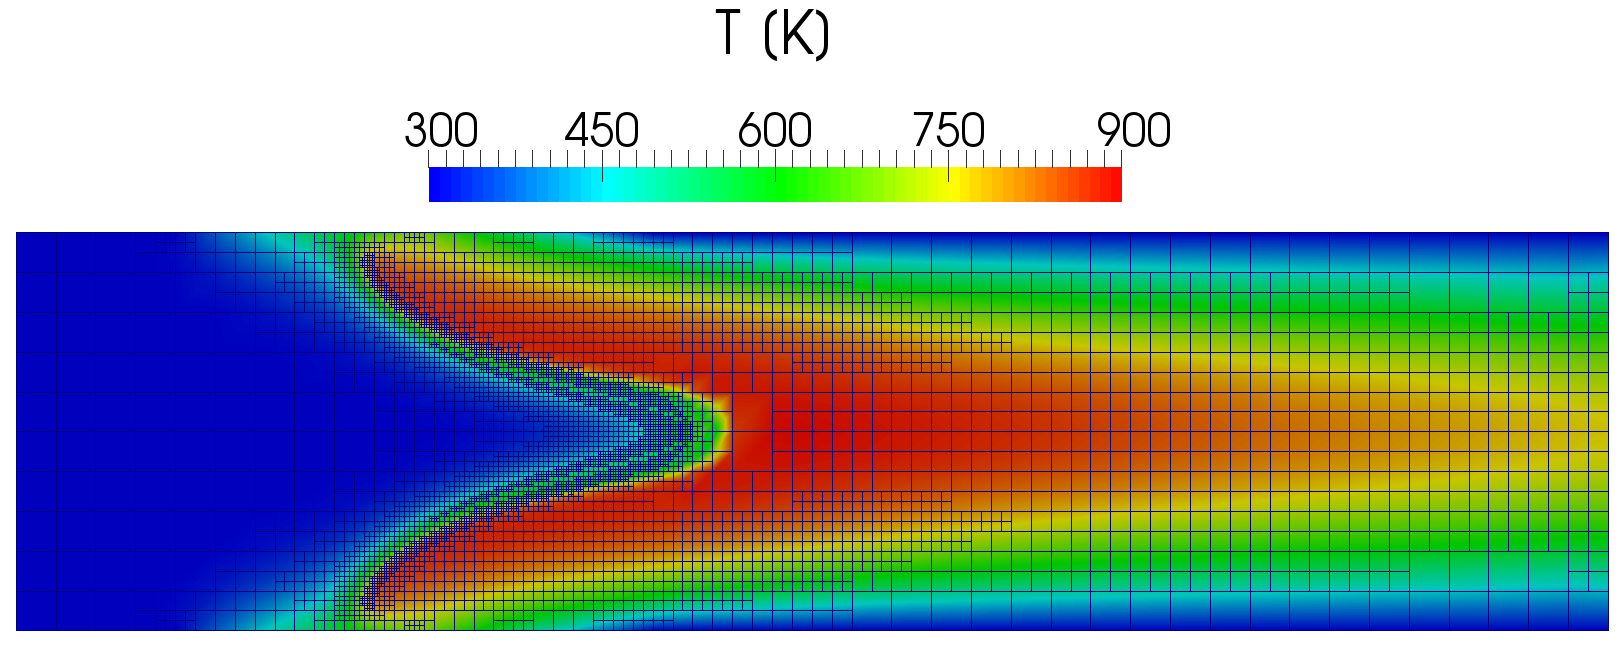
\includegraphics[width=0.9\textwidth]{figs/flame_grins_2}
    \caption{Two-dimensional confined laminar flame calculation using
      stabilized finite element methods and adaptive mesh
      refinement. Generated using the GRINS multiphysics FEM
      framework~\cite{GRINSPaper}.}
    \label{amr_flame}
 \end{figure}
